\setlength{\footskip}{8mm}


\chapter{Methodology}
\label{ch:methodology}

%\section{Methodology}
In this study, we conducted a comprehensive comparison of three object detection algorithms: YOLO (You Only Look Once), Faster R-CNN (Region-based Convolutional Neural Network), and GCN (Graph Convolutional Network) with an adaptive deformation model. The objective was to evaluate their performance in the context of text detection tasks. 

Firstly, we implemented and trained the YOLO model, which excels in real-time detection. However, we found that YOLO struggled to accurately capture multi-oriented and arbitrary-shaped text instances, which are commonly encountered in text detection scenarios. 

Subsequently, we explored the Faster R-CNN framework, known for its exceptional accuracy and ability to handle complex objects. The two-stage architecture of Faster R-CNN, consisting of a region proposal network (RPN) and a detection network, proved to be effective in capturing text instances with arbitrary shapes and orientations. Faster R-CNN exhibited superior performance in localizing and recognizing text, surpassing YOLO in this aspect.

To further enhance the detection capabilities, we incorporated a GCN with an adaptive deformation model. This approach leveraged the graph structure of text instances, capturing the relationships and deformations within the text regions. The GCN's ability to model dependencies among neighboring pixels and exploit contextual information significantly improved the accuracy of text detection, particularly for complex cases involving deformations and variations in text shape.

Through extensive experimentation and evaluation on diverse datasets, we compared the performance of YOLO, Faster R-CNN, and GCN with adaptive deformation. The results demonstrated that the combination of Faster R-CNN and GCN with adaptive deformation achieved the highest accuracy and robustness in text detection tasks, outperforming both YOLO and standalone Faster R-CNN models.

By conducting this comparative analysis, we provide valuable insights into the strengths and limitations of YOLO, Faster R-CNN, and GCN for text detection. The findings highlight the importance of considering the specific characteristics and challenges of text instances and the effectiveness of combining object detection algorithms with graph-based models to improve detection performance in complex scenarios.

\section{YOLO}
YOLO (You Only Look Once) is primarily designed for general object detection, it can also be applied to text detection tasks with some modifications. In the context of text detection, YOLO is utilized to locate and recognize textual content within images. Similar to its usage in object detection, YOLO divides the input image into a grid and predicts bounding box coordinates and class probabilities for each grid cell. However, to adapt YOLO for text detection, certain considerations need to be taken into account. Basic architecture of YOLO is shown below in Figure~\ref{YOLO-Architecture}

\begin{figure}[htp]
  \centering
  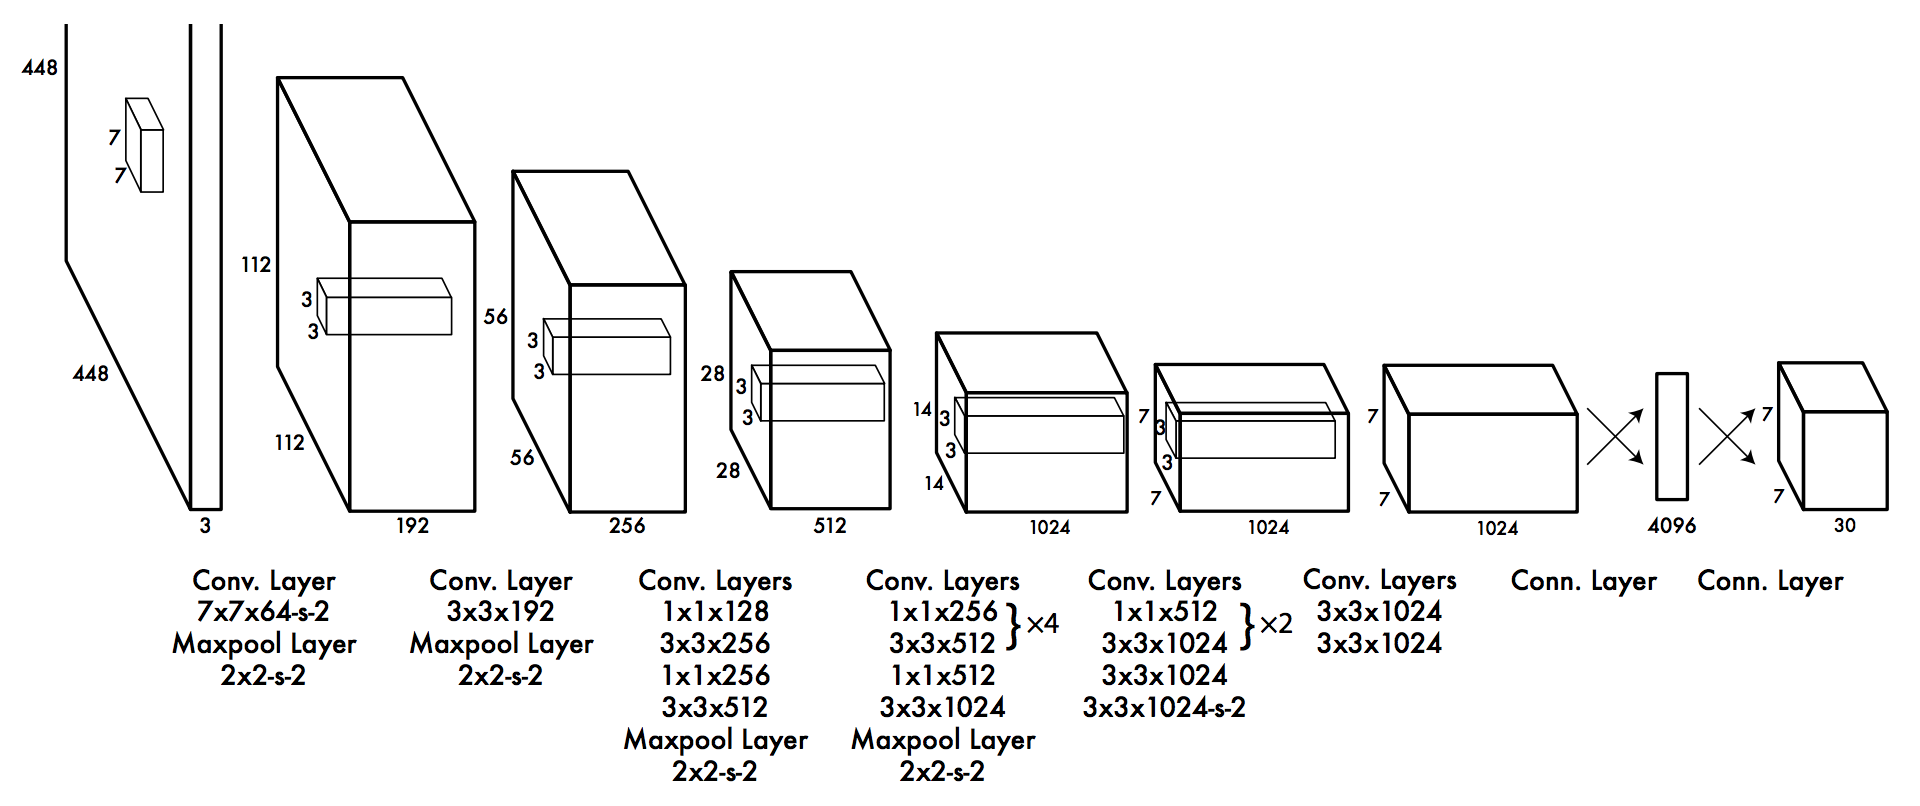
\includegraphics[width=6in]{ITU-Thesis-LaTeX-Template-Updated/figures/yolo_arch.png}
  \caption[YOLO Architecture]{YOLO Architecture 
           Reprinted from the work of Joseph et al.\ (2016).\cite{yolo}}
  \label{fig:YOLO-Architecture}
\end{figure}

\FloatBarrier

To apply YOLO for text detection, the training data should be carefully prepared to include text instances annotated with bounding boxes. This annotated dataset should cover various text sizes, orientations, and styles that are representative of the target application. During training, the YOLO model is trained to recognize and localize text regions by adjusting the network parameters through backpropagation and gradient descent optimization.

When using YOLO for text detection, it is important to address some challenges specific to text. These include handling multi-oriented text (text with non-horizontal orientations), dealing with text of varying aspect ratios, and accurately detecting small-sized text instances. Special techniques can be employed to preprocess the text data, such as applying rotation and perspective transformations to augment the dataset and improve the model's ability to handle multi-oriented and arbitrary-shaped text.

By adapting YOLO for text detection, it becomes possible to efficiently and accurately locate and recognize text within images. The grid-based approach of YOLO allows for real-time processing, making it suitable for applications where fast text detection is required, such as document analysis, OCR (Optical Character Recognition), or text extraction from images. However, it is important to note that while YOLO can be effective for text detection, there may be alternative approaches specifically designed for text-related tasks, such as algorithms that incorporate textual information or utilize graph-based representations to capture the structural relationships between text elements.

\section{Faster R-CNN (Region-based Convolutional Neural Network)}
Faster R-CNN (Region-based Convolutional Neural Network) is a popular object detection framework known for its exceptional accuracy in localizing and classifying objects. Unlike YOLO, which performs detection in a single pass, Faster R-CNN adopts a two-stage approach. It consists of a region proposal network (RPN) that generates potential object proposals and a detection network that refines these proposals and assigns class labels. Below is a picture(~\ref{fig:faster-Architecture} showing how FasterRCNN works: 

\begin{figure}[htp]
  \centering
  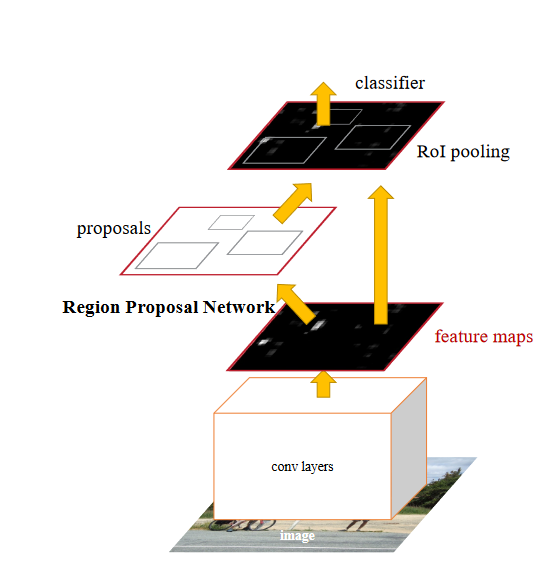
\includegraphics[width=5.65in]{ITU-Thesis-LaTeX-Template-Updated/figures/c1.png}
  \caption[FasterRCNN Architecture]{Faster R-CNN Architecture 
           Reprinted from the work of Shaoqing et al.\ (2016).\cite{faster}}
  \label{fig:faster-Architecture}
\end{figure}

\FloatBarrier

When it comes to text detection, Faster R-CNN demonstrates distinct advantages over YOLO. Text instances often exhibit variations in scale, aspect ratio, and orientation, making them more challenging to detect accurately. Faster R-CNN's two-stage architecture allows it to handle such complexities effectively. The RPN generates region proposals that are better suited for capturing text regions with varying scales and orientations. Moreover, the subsequent detection network refines these proposals and assigns precise bounding box coordinates, leading to improved localization accuracy. The ability of Faster R-CNN to adaptively adjust the region proposals to match the characteristics of text instances makes it particularly well-suited for text detection tasks.

YOLO is known for its real-time detection capabilities, performing object detection in a single pass. It divides the input image into a grid and predicts bounding box coordinates and class probabilities for each grid cell. However, YOLO's grid-based approach and fixed aspect ratios can limit its effectiveness in capturing arbitrary-shaped and multi-oriented text instances. The fixed grid cells and aspect ratios may not align well with the diverse shapes and orientations commonly found in the text, leading to challenges in accurate localization and recognition.

On the other hand, Faster R-CNN addresses these limitations by adopting a two-stage approach. It consists of a region proposal network (RPN) that generates potential object proposals and a subsequent detection network that refines them and assigns class labels. This architecture allows Faster R-CNN to adaptively adjust the region proposals based on the characteristics of the objects, including arbitrary-shaped and multi-oriented text. The RPN can generate more flexible and precise proposals that align with the varying shapes and orientations of text instances, leading to improved detection accuracy.

In the context of arbitrary-shaped and multi-oriented text detection, Faster R-CNN surpasses YOLO by leveraging its two-stage architecture, which enables better handling of these complex text instances. The region proposal stage in Faster R-CNN can generate more accurate proposals that align with the diverse shapes and orientations of text, providing a strong foundation for subsequent detection and recognition. As a result, Faster R-CNN is considered a better approach for capturing arbitrary-shaped and multi-oriented text compared to YOLO.

It is worth noting that both YOLO and Faster R-CNN have their own strengths and weaknesses and their suitability depends on the specific requirements of the text detection task. While YOLO excels in real-time detection and overall object detection scenarios, Faster R-CNN's ability to handle complex text shapes and orientations makes it a preferred choice for tasks involving arbitrary-shaped and multi-oriented text detection.

Despite its strengths, Faster R-CNN also has its limitations. One primary drawback is its computational complexity. The two-stage process involving region proposal and detection networks can be computationally intensive, resulting in slower inference speeds compared to YOLO. Additionally, Faster R-CNN may struggle with detecting small-sized text instances due to the limitations of anchor-based methods in capturing fine-grained details. Furthermore, occlusions and overlapping text regions can pose challenges for Faster R-CNN, as the region proposal stage may struggle to generate accurate proposals in such scenarios. Despite these limitations, Faster R-CNN's superior accuracy and robustness in text detection make it a favored choice in applications where precise localization and classification of text are crucial.

\section{Our Framework}

\begin{figure}[htp]
  \centering
  
\includegraphics[width=6in]{ITU-Thesis-LaTeX-Template-Updated/figures/TextBPN - high quality.png}
  \caption[Our Framework]{Overview of our methodology}
  \label{fig:Our Framework}
\end{figure}

\FloatBarrier
{
The methodology of our approach, depicted in Figure ~\ref{fig:Our Framework}, begins with the adoption of the ResNet-50 model \cite{resnet} for feature extraction. To preserve spatial resolution and leverage multi-level information, we employ a multi-level feature fusion strategy, inspired by FPN \cite{fpn}, as illustrated in Figure 3.3. 

The core component of our method is the boundary proposal model, which consists of multi-layer dilated convolutions. This model utilizes the shared features to perform text pixel classification, generate the distance field, and direction field \cite{textfield}. These fields provide crucial information for producing coarse boundary proposals. Each proposal comprises N points, representing a potential text instance.

To refine the initial coarse proposals, we introduce an adaptive boundary deformation model. This model performs iterative boundary deformations to obtain more accurate text boundaries, guided by prior information such as the classification map, distance field, and direction field.

In summary, our methodology involves feature extraction using ResNet-50, multi-level feature fusion, the boundary proposal model with multi-layer dilated convolutions, generation of coarse boundary proposals using classification, distance, and direction fields, and iterative boundary deformation for refining the proposals using prior information.}


 \section{Boundary Proposal Model}
 The proposed method incorporates the Feature Pyramid Network (FPN) and multi-layer dilated convolutions. FPN captures multi-scale information and ensures robust feature representation, while dilated convolutions capture contextual details and preserve spatial information. This integration enables accurate text detection for various text sizes and shapes. The method generates classification, distance field, and direction field maps to delineate text regions, provide boundary distance information, and indicate text pixel directions. This can be seen in Figure~\ref{fig:BPN}. By leveraging FPN and dilated convolutions, the approach achieves accurate and robust text detection, accommodating diverse text characteristics.
 
\begin{figure}[htp]
  \centering
  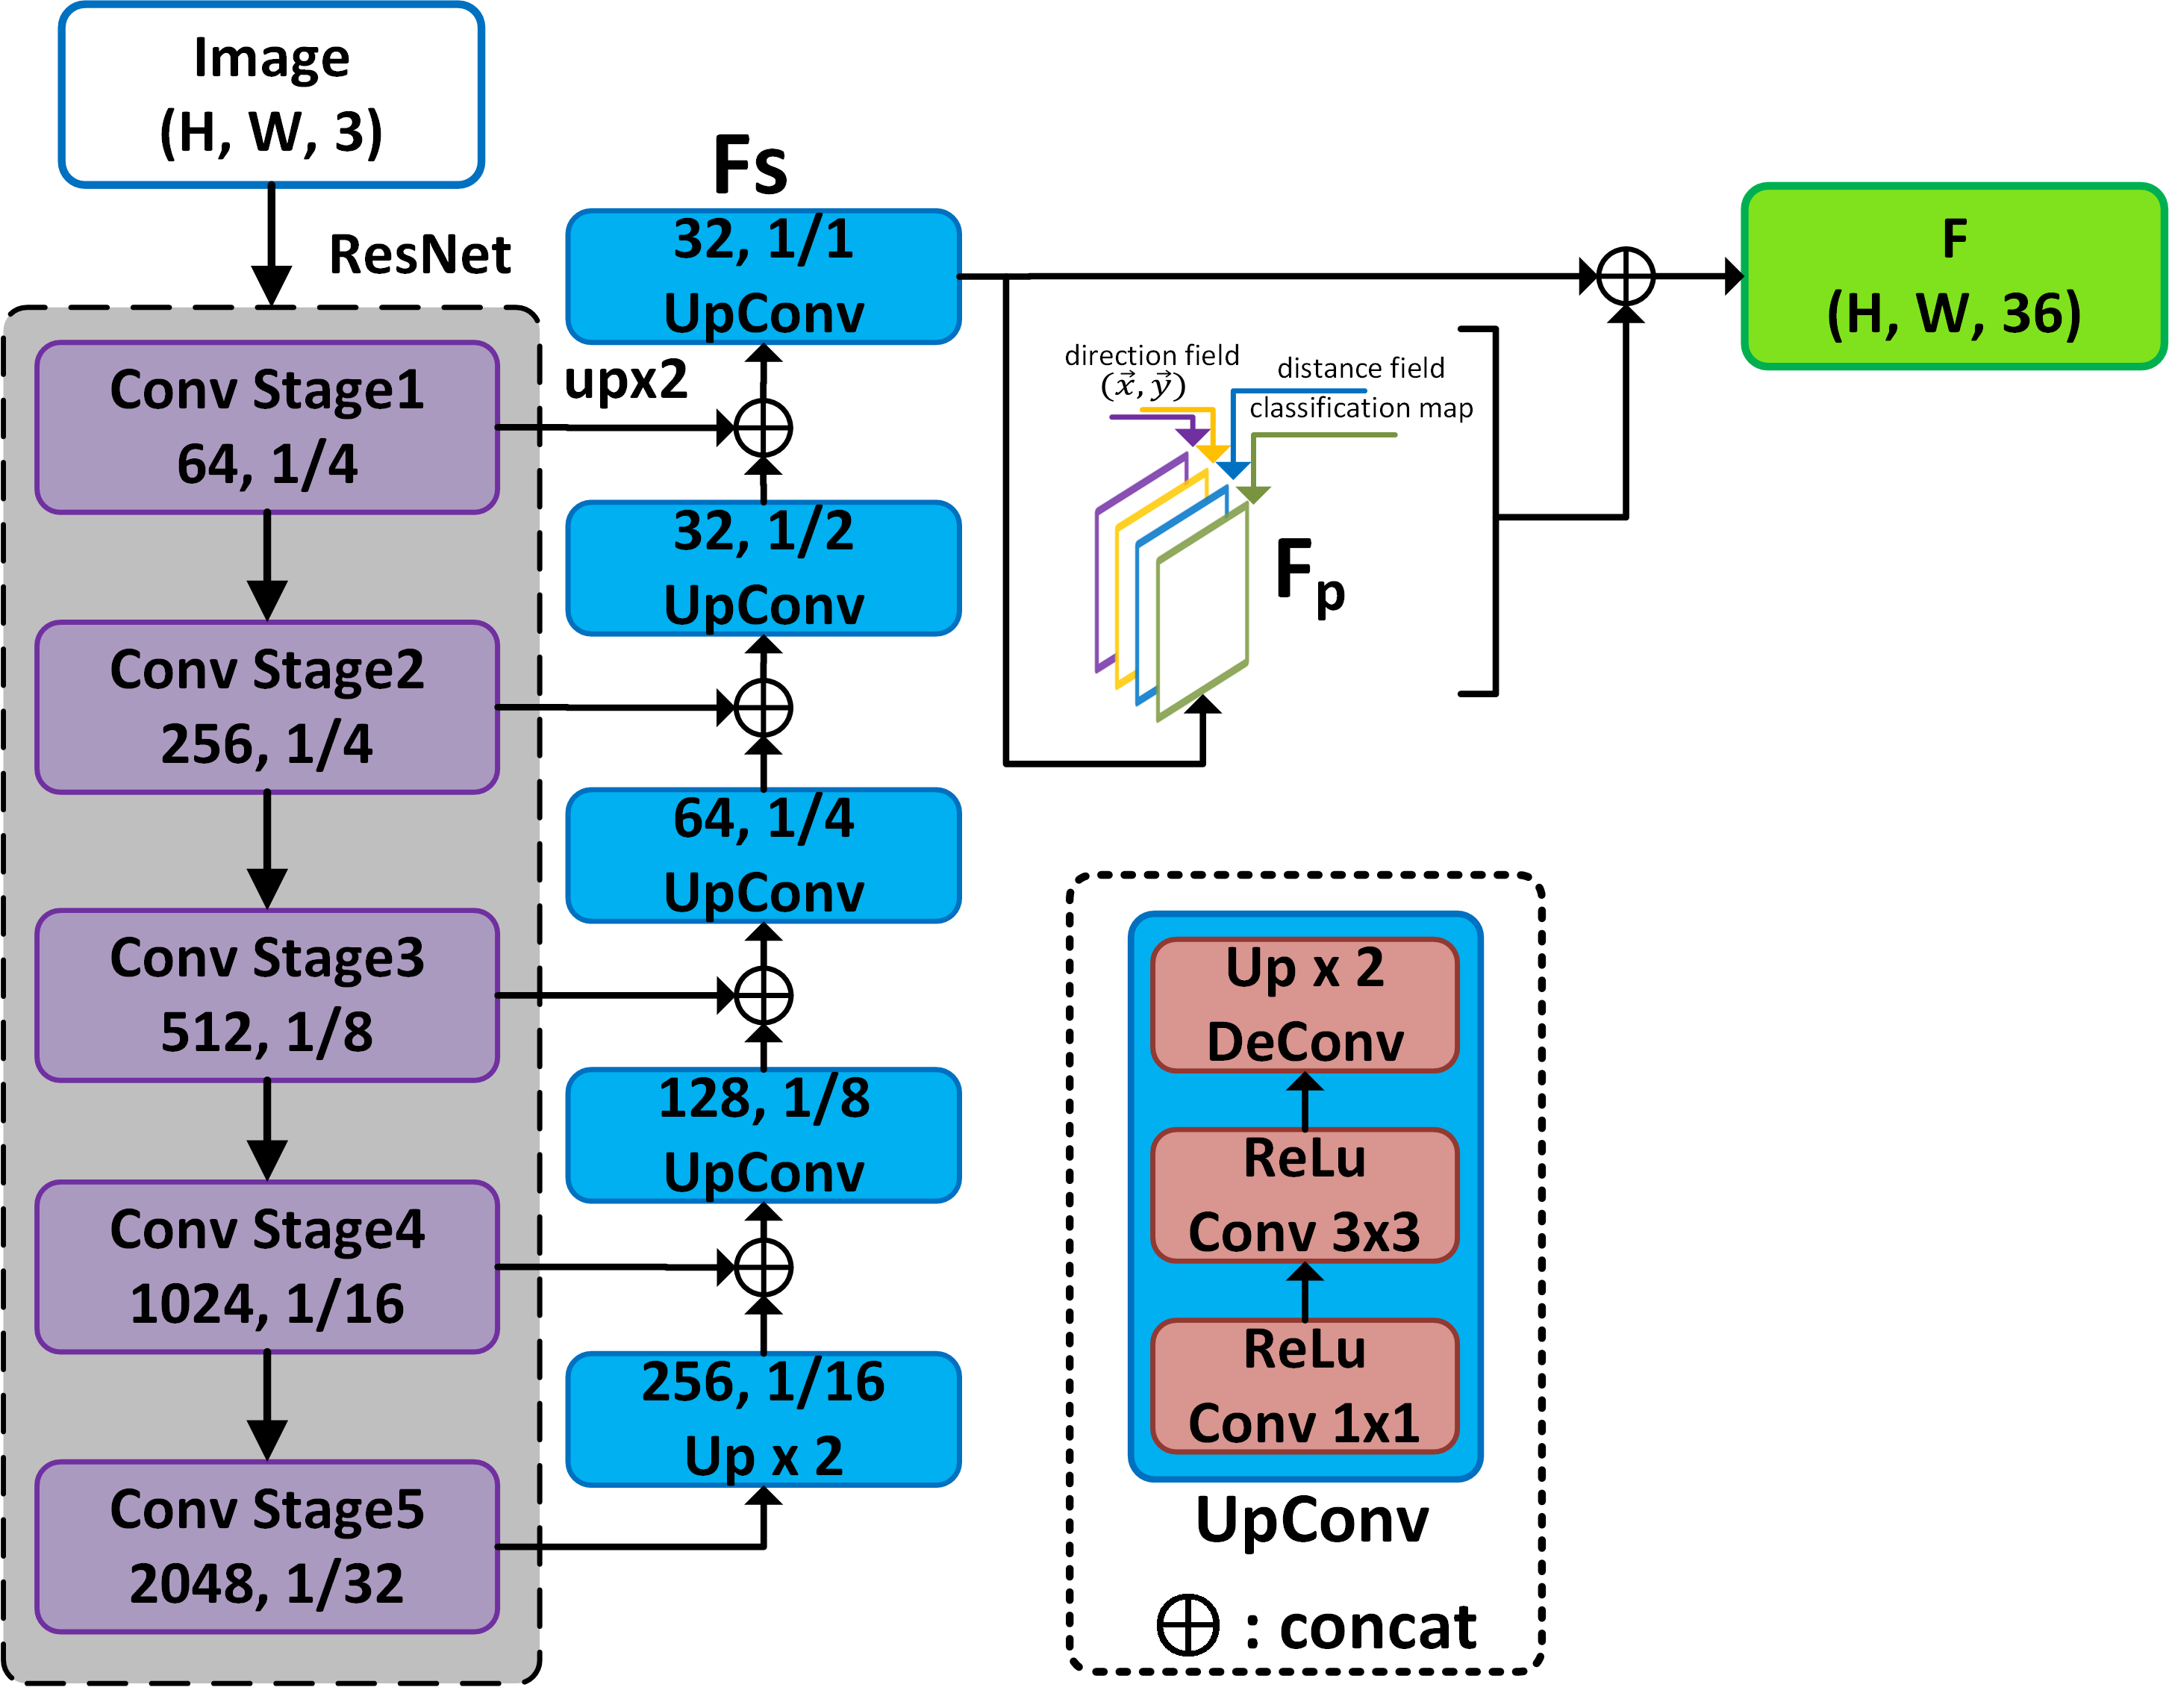
\includegraphics[width=5.65in]{ITU-Thesis-LaTeX-Template-Updated/figures/bpn.png}
  \caption[Boundary Proposal Model]{The architecture of shared convolutions depicting the fusion of shared features (Fs) and prior information (Fp) including the classification map, distance field, and direction field.}
  \label{fig:BPN}
\end{figure}

\FloatBarrier
\subsection{Feature Pyramid Network (FPN)}
The Feature Pyramid Network (FPN) is an architecture that addresses the challenge of detecting objects at different scales in computer vision tasks. It creates a pyramid-like structure of feature maps by leveraging features from multiple levels of a convolutional neural network. The network combines a top-down pathway for upsampling and a bottom-up pathway for downsampling. The fusion of feature maps from different levels through lateral connections preserves fine-grained details and captures both local and global context. In the context of text detection, FPN enables the model to handle varying sizes of text instances and capture both fine details and overall context, enhancing accuracy and robustness.
\subsection{Dilated Convolutions}
Dilated convolutions, also known as atrous convolutions, play a crucial role in improving text detection methodologies. These convolutions introduce gaps or dilations between the values in the convolutional kernel, which expands the receptive field of the model without increasing the number of parameters or layers.

One of the key benefits of dilated convolutions in text detection is the increased receptive field. By adjusting the dilation rate, the model can capture contextual information from a wider area surrounding each pixel. This is particularly useful for detecting longer text instances or considering the context of neighboring characters, leading to improved accuracy.

Another advantage of dilated convolutions is the preservation of spatial resolution. Unlike pooling or down-sampling operations that reduce the resolution, dilated convolutions maintain high-resolution feature maps. This is crucial in text detection tasks where fine details and precise localization are essential for accurate results.

Dilated convolutions excel at handling variable text sizes. In natural scenes, text instances can vary significantly in size. Dilated convolutions adapt to different text scales without the need for multiple layers or explicit resizing operations. This flexibility allows the model to effectively detect text instances of various sizes within the same image.

Efficient modeling is another strength of dilated convolutions. They offer a computationally efficient solution for capturing long-range dependencies and global context. By expanding the receptive field, the model can leverage contextual information without significantly increasing the computational complexity, resulting in improved efficiency and speed in text detection.

Overall, dilated convolutions enhance the ability of text detection models to capture contextual information, handle varying text sizes, and preserve spatial resolution. These benefits contribute to improved accuracy, robustness, and efficiency in detecting text instances in natural scenes.
\begin{figure}[t]
  \centering
  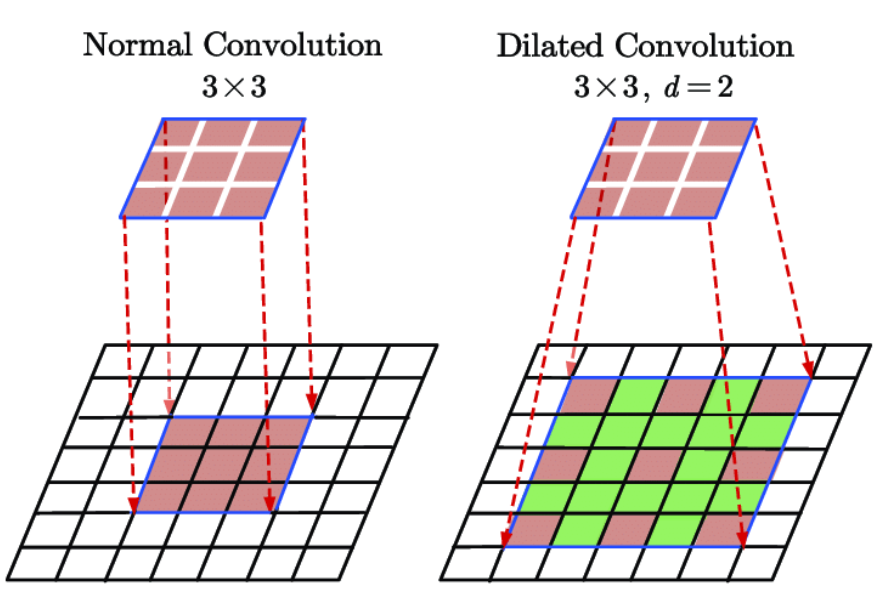
\includegraphics[width=5.65in]{ITU-Thesis-LaTeX-Template-Updated/figures/dilated.png}
  \caption[Dilated Convolution]{The illustration of the 2D dilated convolution with spatial size of 3×3 and dilation factor of 2. Both the non-dilated and 2-dilated convolutions have the same number of parameters, whereas the dilated convolution has a larger receptive field.}
  \label{fig:Dilated-Convolution}
\end{figure}

\FloatBarrier

\subsection{Feature Extraction}
The proposed method leverages the integrated architecture of the Feature Pyramid Network (FPN) and multi-layer dilated convolutions to extract three key features: the direction field, the distance field, and the confidence map. These features play a vital role in accurately delineating and characterizing text regions within the images.
\subsubsection{classification map}
The classification map assigns a classification confidence (text/non-text) to each pixel, similar to other text detection methods \cite{long2020textsnake}\cite{zhang2020deep}\cite{zhou2017east}. 

\subsubsection{Direction Field Map(V)}
In \cite{textfield}\cite{wan2020superbpd}The direction field map (V) consists of two-dimensional unit vectors (→x, →y), indicating the direction from each text pixel towards its nearest pixel on the boundary (pixel-to-boundary). For a given pixel p within a text instance T, its nearest pixel on the text boundary, denoted as Bp, is determined. A unit vector Vgt(p) is then computed to point away from the text pixel p towards Bp. This vector is calculated using the formula:

\begin{equation}
    \label{eqn:Text and non-text separation Method}
 V_{gt}(p) =
\begin{cases}
-\frac{\overrightarrow{Bp}}{\left|\left|\overrightarrow{Bp}\right|\right|}, & \text{if } p \in T \\
(0, 0), & \text{if } p \notin T
\end{cases}
\end{equation}

Here, Bp represents the distance between Bp and the text pixel p, and T represents the set of all text instances in an image. For pixels outside the text area (p $\not\in $ T), we represent them with the vector (0, 0). The unit vector $ V_gt(p) $ encodes both the relative location of p inside T and highlights the boundary between adjacent text instances. It also provides information about the direction for boundary deformation.

\subsubsection{Distance Field Map(V)}
In addition to the direction information, the distance field map (D) is crucial for boundary deformation. The distance field map represents a normalized distance from each text pixel p to its nearest pixel Bp on the text boundary. The normalized distance is defined as:

\begin{equation}
D_{gt}(p) = 
\begin{cases}
\frac{\left|\left|\overrightarrow{Bp}\right|\right|}{L}, & \text{if } p \in T \\
0, & \text{if } p \notin T
\end{cases}
\end{equation}

For pixels outside the text area (p $\not\in$ T), the distance is set to 0. The scale of the text instance T, denoted as L, is defined as the maximum distance value among all text pixels in T. where L is calculated as

\begin{equation}
L = \max(D_{gt}(p));  {p \in T}
\end{equation}

The distance field map Dgt(p) not only encodes the relative distance of p inside T and highlights the boundary between adjacent text instances but also provides relative distance information for boundary deformation.

Using the distance field map (D), candidate boundary proposals can be generated by applying a fixed threshold (thd) to the predicted distance, as depicted in Figure 4 (b). However, these proposals may include false detections. To mitigate this, the average confidence of each candidate boundary proposal is calculated based on the classification map. Proposals with low confidence (below a threshold ths) are then removed, as shown in Figure 4 (c) and (d). This step helps to refine the boundary proposals and remove false detections.

By incorporating these features into the text detection process, the proposed method benefits from a comprehensive understanding of the text regions. The direction field captures the directional cues, the distance field encodes the relative distances, and the confidence map provides pixel-wise classification confidence. Together, these features enhance the accuracy and robustness of text detection, enabling more precise localization and analysis of text instances within images.

\begin{figure}[htp]
  \centering
  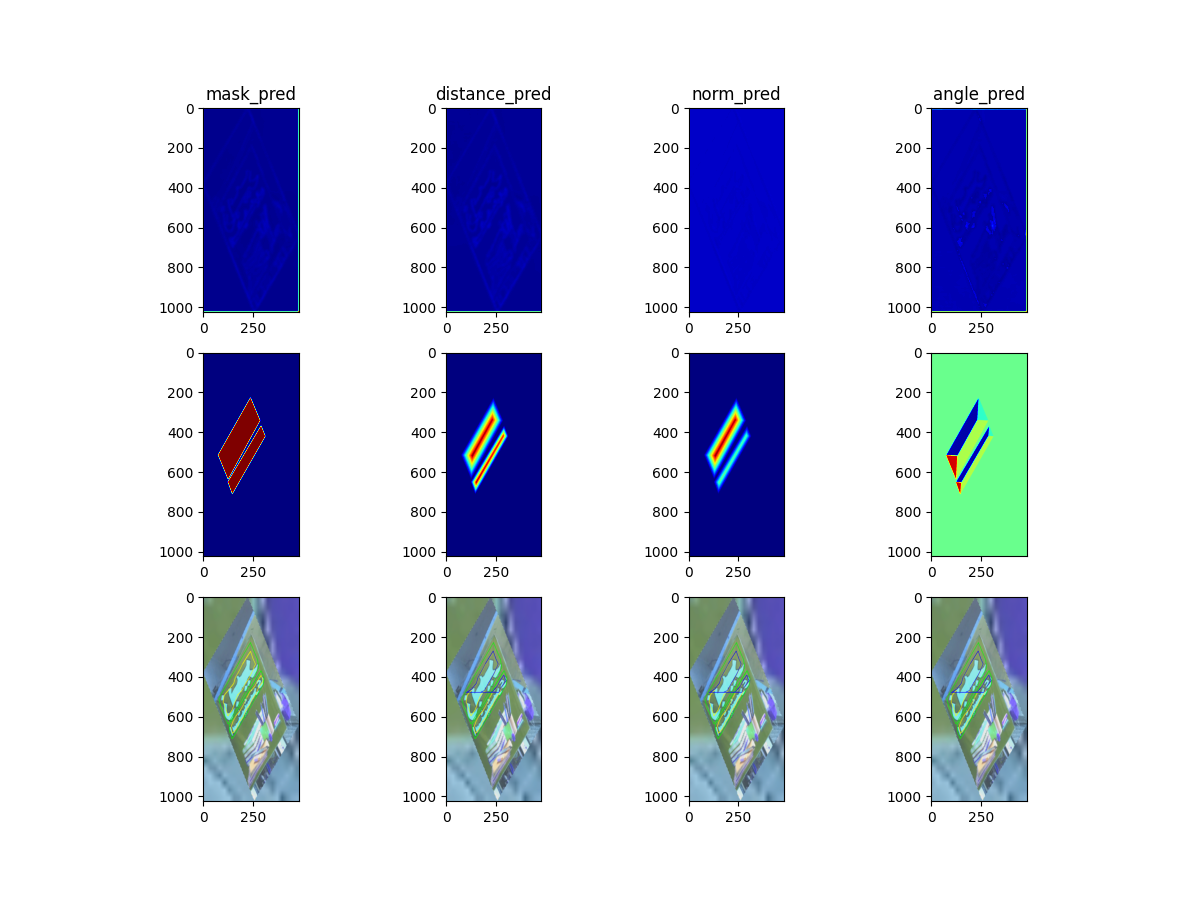
\includegraphics[width=6in]{ITU-Thesis-LaTeX-Template-Updated/figures/2.png}
  \caption[Boundary Proposal Features generation]{Boundary proposal generation illustrating the generation of initial candidate regions using the classification, distance, and direction fields.}
  \label{fig:mesh-feature}
\end{figure}

\section{Adaptive Boundary Deformation}
Motivated by interactive annotation techniques used in object segmentation and instance segmentation methods, we propose a novel approach for arbitrary shape text detection. Our method involves deforming a boundary proposal to accurately delineate the text boundary. Building upon the work of \cite{acuna2018efficient} and \cite{ling2019fast}, which model the sequence of vertices in an object's polygon and treat control point locations as continuous random variables, we introduce a Graph Neural Network that leverages image evidence to predict per-vertex offsets pointing to the text boundary. Additionally, we draw inspiration from DeepSnake \cite{peng2020deep}, which employs circular convolutions with multi-layer 1-D convolutions for object segmentation. However, these existing methods primarily focus on individual topology or sequence context, which may not be optimal for text detection. Existing methods in text detection often focus on either individual topology context or sequence context, which is not fully satisfactory for accurate text detection. However, considering the unique properties of texts, it is crucial to take into account both the topology context and the sequence context simultaneously. Both of these contexts play significant roles in enhancing the performance of text detection algorithms.

To facilitate batch processing, we uniformly sample N control points for each boundary proposal. These control points form a closed polygon, capturing both the topology context and sequence context of the proposal. To fully exploit these contexts, we introduce an adaptive boundary deformation model combined with Graph Convolutional Networks (GCN) and Recurrent Neural Networks (RNN). This model enables efficient feature learning and iterative boundary deformation, leading to the refinement of coarse text boundaries.

\subsection{Feature Extraction and Construction}
For each control point in the boundary proposal, we extract feature vectors that include shared features obtained from a CNN backbone and prior features such as pixels classification, distance field, and direction field. The feature vector for a control point cpi is constructed as follows:

\begin{equation}
f_i = \text{concat}{Fs(x_i, y_i), Fp(x_i, y_i)}
\end{equation}

where $F_s(x_i, y_i)$ and $F_p(x_i, y_i)$ represent the shared features and prior features computed by bilinear interpolation, respectively.
\subsubsection{Bilinear Interpolation}
Bilinear interpolation is a technique used to estimate values within a grid based on known values at grid points. It is commonly used in computer vision and image processing applications, including feature extraction and image resizing.

In the context of the boundary refinement model, bilinear interpolation is employed to compute the shared features $(F_s) $ and prior features $(F_p)$ for each control point. These features are obtained from a CNN backbone and contain important information about the corresponding locations in the feature map.

The process of bilinear interpolation involves calculating a weighted average of the known values surrounding the desired location. Specifically, for a given control point at coordinates (x, y), bilinear interpolation considers the four nearest grid points in the feature map: (x1, y1), (x1, y2), (x2, y1), and (x2, y2), where x1 $\leq$ x $\leq$ x2 and y1 $\leq$ y $\leq$ y2.

Let's understand it with an example;
Consider a set of data coordinates (xk, yk) that define the positions of four points: Q11, Q21, Q12, and Q22. These points represent known values in the grid. Now, suppose we have a new point P with coordinates (x, y) that lies between the xk and yk points. By applying bilinear interpolation, we can calculate the value of point P based on the values of the surrounding points Q11, Q21, Q12, and Q22 as shown in Figure 3.7. Bilinear interpolation takes into account the distances between the known points and the target point P to determine an interpolated value that provides a smooth and continuous estimation within the grid.

\begin{figure}[htp]
  \centering
  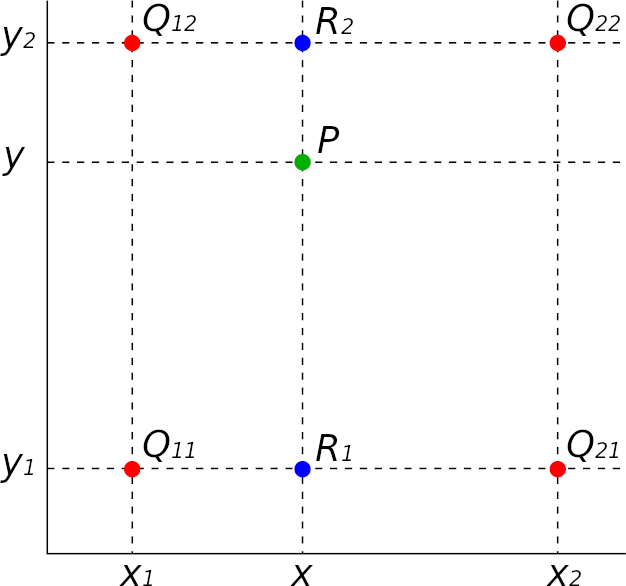
\includegraphics[width=2.2in]{ITU-Thesis-LaTeX-Template-Updated/figures/bilinear.png}
  \caption[Bilinear Interpolation]{Bilinear Interpolation Example.}
  \label{fig:Bilinear Interpolation}
\end{figure}

To find point P(x, y) through biliear interpolation we need to perform the following steps:

    two linear interpolations along the x-axis, finding intermediate points R1 and R2
    one linear interpolation along the y-axis, finding point P

As you can see, bilinear interpolation consists of linear interpolation along both axes, two linear interpolations along x-axis and one linear interpolation along y-axis.

Point R1(x, y) is defined as:
\begin{equation}
  R1(x, y) = Q11 · (x2 – x) / (x2 – x1) + Q21 · (x – x1) / (x2 – x1)
\end{equation}

Point R2(x, y) is defined as:
\begin{equation}
R2(x, y) = Q12 · (x2 – x) / (x2 – x1) + Q22 · (x – x1) / (x2 – x1)
\end{equation}

The interpolated point P(x, y) is defined as:
\begin{equation}
P(x, y) = R1 · (y2 – y) / (y2 – y1) + R2 · (y – y1) / (y2 – y1) 
\end{equation}

By applying bilinear interpolation, the shared features and prior features are computed at each control point, allowing for the construction of the feature vectors (f\textsubscript{i}) used in the boundary refinement process.

Overall, bilinear interpolation enables the interpolation of values within a grid, providing smooth and continuous features for each control point in the boundary proposal. This interpolation process enhances the representation of features and contributes to the accurate refinement of text boundaries.

\subsection{Encoder-Decoder Architecture}
 We present an adaptive deformation model that utilizes an encoder-decoder architecture to enhance the quality of coarse text boundaries. This model is designed to efficiently learn features and iteratively deform the boundaries. The encoder part of the model combines Graph Convolutional Networks (GCNs) and Recurrent Neural Networks (RNNs) to effectively capture and utilize both the boundary topology and sequence context.On the other hand, the decoder part of the adaptive deformation model consists of three layers of 1 × 1 convolutions with Rectified Linear Unit (ReLU) activation function.

 The encoder model can be formulated as:

\begin{equation}
X' = \text{{RN N}}(X) \oplus \text{{GCN}}(X) \oplus \text{{Conv1×1}}(X)
\end{equation}

Here, $\text{{RN N}}(X)$ represents the operation of a recurrent neural network, RNN is a one-layer Bidirectional Long Short-Term Memory (B-LSTM) with a hidden size of 128, $\text{{GCN}}(X)$ represents the operation of a graph convolutional network, and $\text{{Conv1×1}}(X)$ represents the operation of a 1x1 convolution. The $\oplus$ symbol denotes the concatenation operation.

\subsubsection{Graph Convolutional Network}
Graph Convolutional Networks (GCNs) derive their "convolutional" nature from the fact that they learn filters during training, which are typically shared across all locations in the graph. This concept is similar to how convolutional filters are learned in computer vision tasks, where filters are applied to image inputs and shared across all pixel locations. Graph Convolutional Networks (GCNs) have emerged as a powerful technique for analyzing graph-structured data. Unlike traditional convolutional neural networks (CNNs) that operate on regular grid-like data, GCNs can handle irregular and non-grid data represented as graphs as shown in Figure~\ref{fig:GCN}.

\begin{figure}[htp]
  \centering
  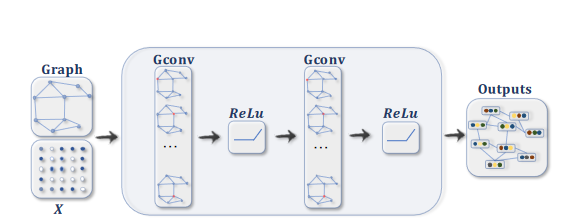
\includegraphics[width=6in]{ITU-Thesis-LaTeX-Template-Updated/figures/GCN.png}
  \caption[The Convolutional Graph Neural Network (ConvGNN)]{The Convolutional Graph Neural Network (ConvGNN) leverages multiple graph convolutional layers to capture the hidden representations of nodes. Each layer aggregates feature information from a node's neighbors, enabling the model to incorporate the influence and interactions between nodes. Non-linear transformations are applied to the aggregated features, introducing non-linearity. By stacking multiple layers, the final hidden representation of each node integrates information from a broader neighborhood, allowing for the learning of complex patterns and higher-order dependencies in the graph structure Reprinted from Zonghan et al.2021\cite{Wu_2021}.}
  \label{fig:GCN}
\end{figure}
\FloatBarrier

A graph is a data structure that consists of a set of vertices (also known as nodes) and a set of edges connecting these vertices. A graph is a way of representing relationships or connections between different elements. Formally, a graph G is defined as G = (V, E), where V represents the set of vertices/nodes, and E represents the set of edges. In the context of GCNs, we define a graph G = (V, E), where each node i is associated with initial node features xi. The input to the GCN model consists of the graph itself and the initial node features X, which is a matrix of size N × D, where N represents the number of nodes and D represents the dimensionality of the node features. The goal of the GCN is to learn representations for each node, and at the final layer, we obtain node representations denoted as Z, which is a matrix of size N × F.

The basic formulation of GCNs can be expressed as follows:

\begin{equation}
H^{(l+1)} = \sigma(AH^{(l)}W^{(l)})
\end{equation}

Here, H(l) represents the node representations at the l\-th layer, $\sigma$(·) denotes a non-linear activation function such as ReLU, A represents the adjacency matrix of the graph, and W(l) represents the trainable weight matrix at the l\-th layer.

To enhance the expressive power of GCNs, more sophisticated forms have been developed. One such form includes the normalization of the adjacency matrix and the addition of identity connections. The formulation is as follows:

\begin{equation}
H^{(l+1)} = \sigma(\tilde{D}^{-\frac{1}{2}}\tilde{A}\tilde{D}^{-\frac{1}{2}}H^{(l)}W^{(l)})
\end{equation}

Here, $\tilde{A}$ is the adjacency matrix of the graph with an added identity matrix I and D is the diagonal matrix containing the node degrees of $\tilde{A}$.

While the original full-batch GCN approach requires computing representations for all nodes in the graph at each GCN layer, this approach can be computationally expensive and memory inefficient, making it challenging to generalize to larger graphs. In recent years, there has been an increase in research that applies convolutional neural networks on graph nodes and operates on neighborhoods of nodes, providing more scalable and efficient solutions for GCN-based models.

\subsubsection{Leveraging Graph Convolutional Networks for Text Detection in Images}
Graph Convolutional Networks (GCNs) have emerged as a potent tool for graph-based data analysis. In this thesis, we harness the power of GCNs to address the challenging task of text detection in images. We introduce the critical concepts of nodes, the adjacency matrix, and the graph convolution operation, which together form the foundation of our methodology.

\paragraph{Graph Construction} \hfill \break 
\textbf{Node Feature Matrix} \hfill \break
At the core of our approach lies the node feature matrix, a foundational element in constructing our graph. This matrix, sized at 32xN, encapsulates the core of our boundary proposal model. Each node within the graph represents a unique region or control point derived from the boundary proposal. These nodes serve as the foundation upon which our GCN orchestrates the symphony of text detection. The node feature matrix, referred to as features, becomes the embodiment of these regions' characteristics and is pivotal in the subsequent stages of our text detection methodology. Here is a example of node in Figure~\ref{fig:nodes}

\begin{figure}[htp]
  \centering
  \begin{minipage}{0.3\textwidth}
    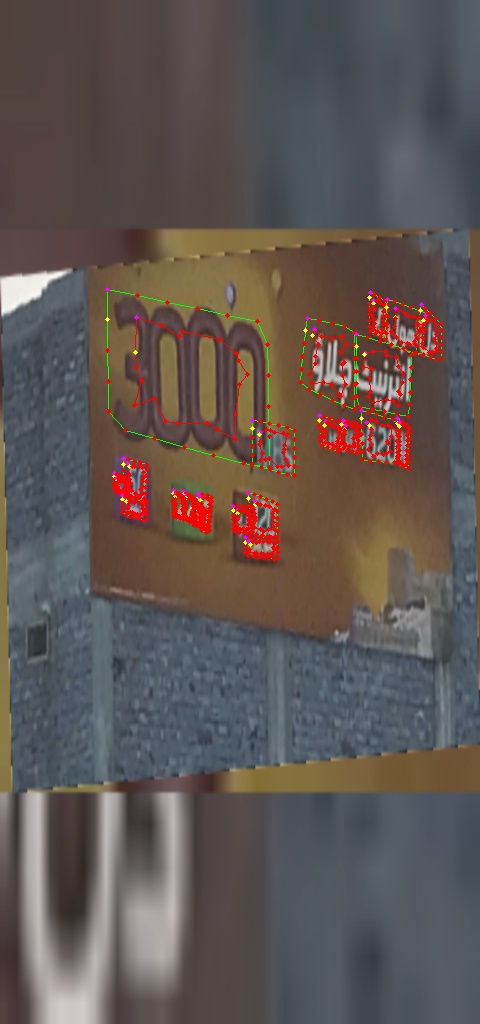
\includegraphics[width=\linewidth]{ITU-Thesis-LaTeX-Template-Updated/figures/458.jpg} 
  \end{minipage}
  \begin{minipage}{0.3\textwidth}
    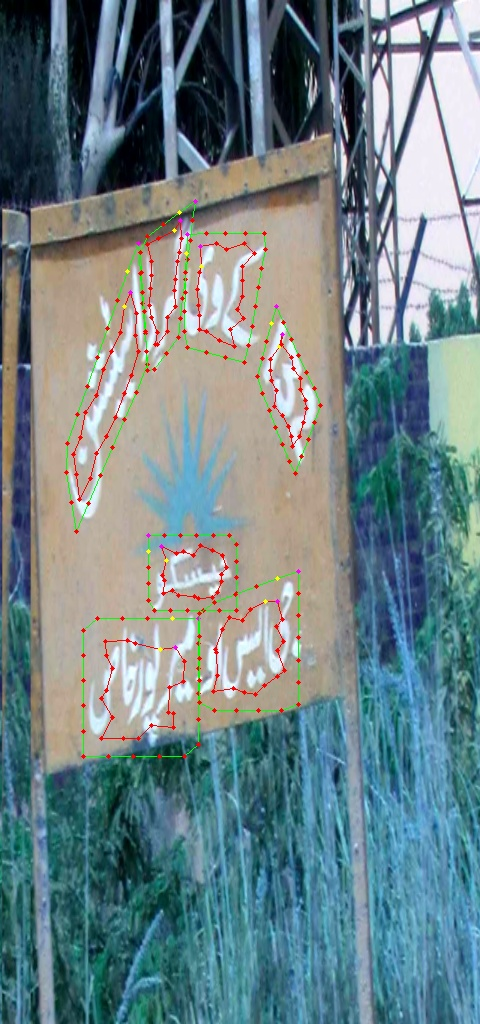
\includegraphics[width=\linewidth]{ITU-Thesis-LaTeX-Template-Updated/figures/581.jpg}
  \end{minipage}
  \begin{minipage}{0.3\textwidth}
    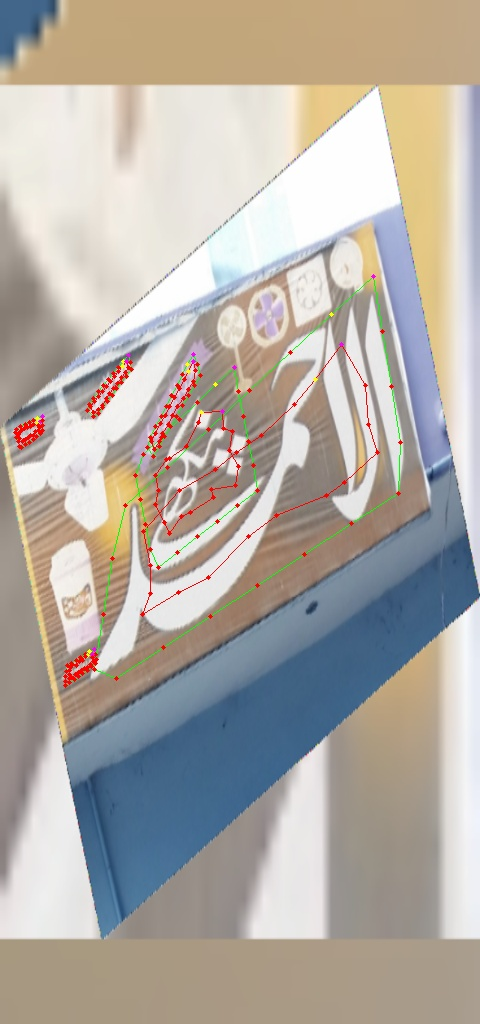
\includegraphics[width=\linewidth]{ITU-Thesis-LaTeX-Template-Updated/figures/503.jpg}    
  \end{minipage}
  \caption[Graph Structure]{Text Boundary for Nodes Generation. }
  \label{fig:nodes}
\end{figure}
\FloatBarrier

\textbf{Adjacency Matrix} \hfill \break
As explained earlier adjacency matrix, denoted as A, is a square matrix of size N x N, where N represents the number of nodes in the graph. Unlike traditional adjacency matrices, which indicate explicit connections between nodes, our approach leverages the adjacency matrix differently.

In our methodology, we employ the adjacency matrix as a guiding structure rather than an explicit connection matrix. It aids in the determination of edge relationships based on specific criteria, such as spatial proximity and other contextual factors. This unique application allows us to create a dynamic and context-aware graph, ideal for text detection tasks. \\

\textbf{Edge Determination} \hfill \break
Edges, the connective threads within our graph, play a pivotal role in capturing relationships and dependencies between nodes. Our edge determination process is meticulously designed to ensure the contextual relevance of these connections. Let's elucidate the concrete steps involved: \\

\textbf{Criteria Definition:} The edge determination process begins with the definition of specific criteria. These criteria, predetermined and carefully considered, form the backbone of our graph's structure. Notably, spatial proximity between control points stands as one of the primary criteria embedded in our code.

\textbf{Edge Score Calculation:} With criteria in place, the code proceeds to compute edge scores for all conceivable pairs of nodes. These scores serve as the quantitative measures of the relationships between nodes. It's essential to emphasize that the formula governing edge score calculation can be customized to suit the unique characteristics of the problem at hand. Moreover, the code boasts the flexibility to fine-tune edge scores based on additional context-specific factors.

\textbf{Thresholding:} To refine the graph's density and connectivity, a judicious thresholding step follows edge score calculation. This step allows for the fine-tuning of the graph's structure by filtering out edges with scores below a designated threshold. The ability to manipulate this threshold empowers us with granular control over the inclusion or exclusion of edges, adapting the graph to the nuances of the text detection task.

\paragraph{Graph Convolution Operation}\hfill \break 
The graph convolution operation forms the core of our text detection methodology. It involves aggregating information from neighboring nodes and updating node features. We provide the mathematical formulation of the graph convolution operation, including the activation function and the weight matrices involved. The symmetric normalized Laplacian matrix is introduced to capture the graph structure and facilitate information propagation.

The graph convolution operation is a fundamental operation in Graph Convolutional Networks (GCNs) that enables information propagation and feature learning on graph-structured data. It operates on the nodes (vertices) and edges of a graph to update the feature representations of each node based on its neighbors.The adjacency matrix, while not representing explicit connections, guides the flow of information during this operation. It helps identify neighboring nodes, facilitating the aggregation process.


Mathematically, the graph convolution operation can be expressed as follows:

\begin{equation}
h_v^{(l+1)} = \sigma\left(\sum_{u \in \mathcal{N}(v)} \frac{1}{\sqrt{|\mathcal{N}(v)||\mathcal{N}(u)|}} \cdot \theta^{(l)} \cdot h_u^{(l)}\right)
\end{equation}

In this equation, $h_v^{(l+1)}$ represents the feature representation of node $v$ at the $(l+1)$-th layer, $\mathcal{N}(v)$ denotes the set of neighboring nodes of $v$, $\theta^{(l)}$ represents the trainable weight matrix at the $l$-th layer, $h_u^{(l)}$ represents the feature representation of node $u$ at the $l$-th layer, and $\sigma$ denotes the activation function. The sum over $u \in \mathcal{N}(v)$ indicates the aggregation of information from neighboring nodes, and the term $\frac{1}{\sqrt{|\mathcal{N}(v)||\mathcal{N}(u)|}}$ is a normalization factor to account for the varying degrees of connectivity between nodes.

Let's break down the components of the graph convolution operation:
\begin{enumerate}
\item Neighborhood Aggregation: The operation iterates over the neighboring nodes u of a given node v and aggregates their feature representations, weighted by the factor $\frac{1}{\sqrt{|\mathcal{N}(v)||\mathcal{N}(u)|}}$. This weight normalization accounts for the varying degrees of connectivity and ensures that the aggregated information is properly scaled.

\item Weight Matrix: The weight matrix $\theta^{(l)}$ is specific to each layer of the GCN and represents the trainable parameters that control the transformation applied to the aggregated features. It maps the aggregated features of the neighbors to the updated feature representation of the central node.

\item Activation Function: The activation function $\sigma$ introduces non-linearity to the graph convolution operation, allowing for the modeling of complex relationships between nodes.

\end{enumerate}

Overall, the graph convolution operation performs a weighted aggregation of features from neighboring nodes and applies a transformation using the weight matrix. This operation allows nodes in a graph to exchange information and update their feature representations based on the features of their neighbors. By stacking multiple layers of graph convolutions, GCNs can capture increasingly complex patterns and dependencies in the graph structure, enabling powerful feature learning and information propagation.

% \paragraph{Utilizing the Spatial Nature of Graph Convolutional Networks for Text Detection}\hfill \break 
% The spatial nature of Graph Convolutional Networks (GCNs) can be effectively utilized for text detection tasks. In the context of text detection, we consider a graph where each node represents a specific region or element in the input image. The goal is to learn discriminative features for accurate text detection.

% To prove the spatial nature of GCNs for text detection, we observe the behavior of information propagation within the network. Each node in the graph passes and receives information to/from its neighboring nodes, simulating a spatial relationship among the regions in the image.

% \paragraph{Graph Construction}\hfill \break 
% In our methodology, we construct a graph to represent the boundary proposals. Each control point within the boundary proposal is considered a node in the graph. The edges of the graph are determined based on the spatial relationships and connectivity between the control points. Specifically, we connect nodes that are spatially close or have significant interactions based on the topology context of the boundary proposal. This tailored graph structure captures the relevant relationships and facilitates the subsequent refinement process.

\paragraph{GCN for Boundary Refinement}\hfill \break 
In our methodology, we utilize GCNs to refine the coarse text boundaries. The GCNs leverage the constructed graph structure to propagate information between control points, capturing the topology context and sequence context of the boundary proposals. This enables efficient feature learning and iterative boundary deformation, leading to the refinement of text boundaries. By incorporating GCNs, our methodology benefits from enhanced feature representation and context-aware refinement, ultimately improving the accuracy and precision of text boundary detection.

By leveraging the power of GCNs and the graph structure, our methodology effectively exploits the interdependencies and spatial relationships between control points in the boundary proposals. This enables more precise and accurate text boundary refinement, enhancing the overall performance of text detection algorithms.


\subsubsection{Recurrent Neural Network}
In our adaptive deformation model, we leverage the power of a Bi-LSTM (Bidirectional Long Short-Term Memory) network as the recurrent neural network component. The Bi-LSTM represents a remarkable advancement in sequence modeling, capable of capturing both past and future context simultaneously. By incorporating this sophisticated architecture, our model gains the ability to exploit the intricate temporal dependencies present in the text detection task. The Bi-LSTM analyzes the input data bidirectionally, allowing it to learn intricate patterns and relationships that may be crucial for accurate and robust boundary deformation. Through its bidirectional nature, the Bi-LSTM provides a comprehensive understanding of the sequential information, empowering our model to make informed and contextually aware decisions during the boundary refinement process.

\paragraph{Bi-LSTM}\hfill \break
A Bidirectional Long Short-Term Memory (Bi-LSTM) is a type of recurrent neural network (RNN) that processes sequential data in both forward and backward directions. It is an extension of the traditional LSTM architecture, which is designed to capture long-term dependencies and handle sequential data.

The Bi-LSTM consists of two LSTM layers, one processing the input sequence in the forward direction and the other in the backward direction. The forward LSTM layer processes the sequence from the beginning to the end, while the backward LSTM layer processes the sequence in reverse order, starting from the last element. By capturing information from both directions, the Bi-LSTM is able to effectively model the dependencies in the sequence.

At each time step, the forward and backward LSTM layers receive the input from the previous time step, as well as their respective hidden states. The hidden states of the forward LSTM layer capture the information from the past, while the hidden states of the backward LSTM layer capture the information from the future. The outputs of the forward and backward LSTM layers at each time step are concatenated to obtain the final output of the Bi-LSTM.

The Bi-LSTM architecture allows the model to capture both local and global dependencies in the input sequence. The forward pass of the Bi-LSTM processes the sequence and generates hidden representations that capture the dependencies up to the current time step, while the backward pass processes the sequence in reverse and captures the dependencies from the future. By combining these representations, the Bi-LSTM can make more informed predictions and better understand the context of the sequential data.

In natural language processing tasks, the Bi-LSTM is often used for tasks such as sentiment analysis, named entity recognition, and machine translation, where understanding the context of the words in a sentence or sequence is crucial. The bidirectional nature of the Bi-LSTM allows it to effectively capture dependencies in both directions, improving the model's ability to capture long-term dependencies and make accurate predictions.

\begin{figure}[htp]
  \centering
  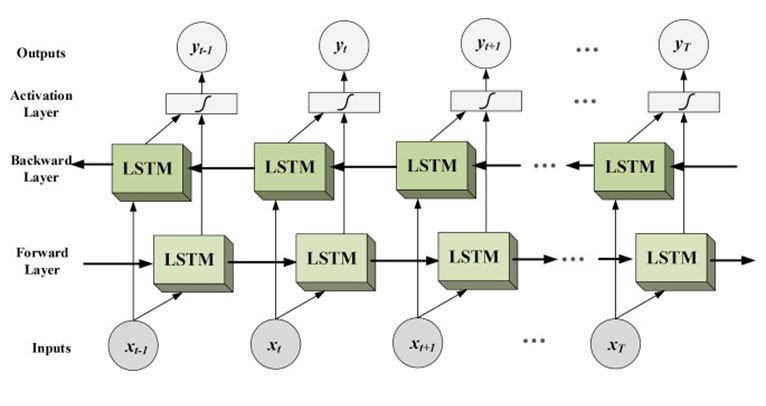
\includegraphics[width=5in]{ITU-Thesis-LaTeX-Template-Updated/figures/bi-lastm.jpg}
  \caption[Bi-LSTM]{Bi-LSTM Architecture}
  \label{fig:Bi-LSTM}
\end{figure}

\paragraph{Bi-LSTM Working}\hfill \break
Let's dive into the working of a Bidirectional Long Short-Term Memory (Bi-LSTM) network, including the mathematical formulation.

The forward LSTM layer computes the hidden states in the forward direction, denoted as $H_f = [h_{1f}, h_{2f}, ..., h_{Tf}]$. Similarly, the backward LSTM layer computes the hidden states in the backward direction, denoted as $H_b = [h_{1b}, h_{2b}, ..., h_{Tb}]$.

The hidden states of the forward LSTM layer are calculated as follows:
$$h_{tf} = \text{LSTM}_f(x_t, h_{t-1f})$$

Similarly, the hidden states of the backward LSTM layer are calculated as follows:
$$h_{tb} = \text{LSTM}_b(x_t, h_{t+1b})$$

\begin{equation}
\begin{aligned}
\text{Forward LSTM Cell:} \\
f_t &= \sigma(W_{xf}x_t + W_{hf}h_{t-1f} + b_f) \\
\tilde{C}_t &= \text{tanh}(W_{cf}x_t + U_{cf}h_{t-1f} + b_c) \\
C_t &= f_t \odot C_{t-1} + \tilde{C}_t \\
o_t &= \sigma(W_{xo}x_t + W_{ho}h_{t-1f} + b_o) \\
h_{tf} &= o_t \odot \text{tanh}(C_t) \\
\\
\text{Backward LSTM Cell:} \\
f_t &= \sigma(W_{xb}x_t + W_{hb}h_{t+1b} + b_b) \\
\tilde{C}_t &= \text{tanh}(W_{cb}x_t + U_{cb}h_{t+1b} + b_c) \\
C_t &= f_t \odot C_{t+1} + \tilde{C}_t \\
o_t &= \sigma(W_{xo}x_t + W_{ho}h_{t+1b} + b_o) \\
h_{tb} &= o_t \odot \text{tanh}(C_t) \\
\end{aligned}
\end{equation}
In the above equations, $\sigma$ represents the sigmoid activation function, $\odot$ represents element-wise multiplication, $W$ and $U$ are weight matrices, $b$ represents bias vectors, and $\text{tanh}$ represents the hyperbolic tangent activation function.
\hfill \break
The outputs of the Bi-LSTM at each time step are obtained by concatenating the forward and backward hidden states:
$$h_t = [h_{tf}, h_{tb}]$$

The Bi-LSTM architecture allows the model to capture both local and global dependencies in the input sequence by considering information from both the past and the future. Bi-LSTM's ability to capture contextual information, handle variable-length sequences, learn effective features, and support iterative refinement makes it a valuable component in text detection models. It allows the model to leverage both local and global contexts, leading to improved accuracy and robustness in detecting text regions in various settings.

\paragraph{GCN and RNN Combination}
The combination of GCN and RNN facilitates feature learning and iterative boundary deformation. GCN enables efficient information propagation and feature extraction by treating the control points as nodes in a graph. This allows the model to capture the connectivity and spatial relationships between the control points, enhancing its understanding of the boundary topology.
RNN, on the other hand, models the sequential nature of the boundary deformation process. By processing the control points in a sequential manner, the model can leverage the sequence context and capture the temporal dependencies between adjacent control points. This enables iterative boundary refinement, improving the accuracy of text boundaries with each iteration.

\subsubsection{Convolution 1x1}

A Conv1×1 layer refers to a convolutional layer with a kernel size of 1×1. Unlike traditional convolutional layers that typically have larger kernel sizes, such as 3×3 or 5×5, a Conv1×1 layer has a kernel size of 1×1.

The inclusion of Conv1×1 convolutions in the text detection framework brings several benefits to improve its performance:

1. Enhanced Feature Representation: Conv1×1 convolutions transform the input feature map and reduce its dimensionality. This process helps in capturing more meaningful and compact representations of the input data. By incorporating Conv1×1 convolutions, the framework can learn more expressive features that are beneficial for distinguishing text regions from the background.

2. Efficient Fusion of Information: The concatenation of Conv1×1 features with GCN and RNN outputs enables the fusion of information from different sources. The Conv1×1 convolutions capture local patterns, while GCN and RNN layers capture graph-based and sequential contextual information, respectively. The fusion of these diverse features helps the model to gain a more comprehensive understanding of the text in the image and improve its ability to detect text accurately.

3. Adaptive Deformation and Boundary Refinement: The three-layer 1 × 1 convolutions in the decoder play a crucial role in predicting offsets between control points and target points. This iterative boundary deformation process, guided by Conv1×1 convolutions, allows for refining the coarse text boundaries and achieving more accurate text detection. The Conv1×1 convolutions contribute to the refinement process by learning to adjust the boundaries based on the specific characteristics of the text in the image.

Overall, the incorporation of Conv1×1 convolutions in the text detection framework benefits the system by enhancing feature representation, facilitating efficient information fusion, and enabling adaptive deformation and boundary refinement. These improvements contribute to the overall performance of the framework, leading to more accurate and robust text detection in natural images.

\section{Implementation Details}
In our experimental setup, the initial phase involves pre-training the network on SynthText using a single epoch. During this pre-training, images are subjected to random cropping and resizing, resulting in a uniform size of 512 × 512. The training process utilizes the Adam optimizer with a fixed learning rate of 0.001 and mini-batches containing 16 samples.

For fine-tuning, we proceed by randomly cropping the text regions from the images and resizing them to dimensions of 640 × 640. This stage employs a mini-batch size of 12 and continues to use the Adam optimizer. The initial learning rate of 0.001 is subsequently decreased to 0.9 of its original value after every 50 epochs. Data augmentation techniques, including random rotation within the range of -60° to 60° (sampled from a Gaussian distribution), random cropping, and random flipping, contribute to the robustness of the model.

In the inference phase, the aspect ratio of test images is maintained, and they are then resized and padded to a consistent size for testing purposes. Our implementation employs PyTorch 1.7 and Python 3, and the training is executed on a single RTX-3090 GPU, while testing occurs on a single GeForce RTX-2080 GPU, complemented by an Intel Xeon Silver 4108 CPU @ 1.80GHz.

\section{Evaluation Metrics}
Our evaluation strategy employs precision, recall, and the F-score as foundational metrics to thoroughly assess the performance of our text detection methodology. These metrics collectively provide a comprehensive view of the model's ability to accurately identify and localize text instances within images.

\textbf{Precision (P):} Precision quantifies the accuracy of the model's positive predictions. It is calculated using the formula:

\begin{equation}
P = \frac{TP}{TP + FP}
\end{equation}

Where: \\
\begin{itemize}
    \item TP represents the number of true positive predictions.
    \item FP represents the number of instances predicted as positive but are actually negative. \\
\end{itemize}

\textbf{Recall (R):} Recall measures the model's capacity to capture all relevant instances. It is defined as the ratio of true positive predictions to the total actual positives:

\begin{equation}
R = \frac{TP}{TP + FN}
\end{equation}

Where: \\
\begin{itemize}
    \item FN is the number of actual positive instances that the model failed to predict. \\
\end{itemize}

\textbf{F-score:} The F-score, or F1-score, offers a balanced assessment by considering both precision and recall. It is calculated as the harmonic mean of precision and recall:

\begin{equation}
F = \frac{2 \cdot (P \cdot R)}{P + R}
\end{equation}

In summary, precision evaluates the accuracy of positive predictions, recall assesses the comprehensiveness of positive instance identification, and the F-score provides a consolidated measure that considers both false positives and false negatives. By utilizing these metrics, we gain a holistic understanding of our methodology's effectiveness in accurately detecting text instances, guiding potential optimizations and improvements.



% \renewcommand{\algorithmicrequire}{\textbf{Input:}}
% \renewcommand{\algorithmicensure}{\textbf{Output:}}
% \renewcommand{\algorithmicforall}{\textbf{for each}}
% \begin{algorithm}
% \caption{Lame Algorithm}
% \label{lame-algorithm}
% \begin{algorithmic}
%   \REQUIRE $B$: set of all current blobs
%   \REQUIRE $T$: set of all current tracks
%   \REQUIRE $M$: merged track association matrix
%   \ENSURE $\widetilde{T}$: set of all revised tracks
%   \ENSURE $\widetilde{M}$: revised merged track association matrix
%   \STATE $\widetilde{T} \gets \emptyset$; $\widetilde{M} \gets \emptyset$; $L \gets \emptyset$
% %  \STATE \COMMENT{Construct an overlap area matrix between the bounding box of blobs and tracks.}
%   \STATE $A \gets \textsc{Get-Overlap-Area-Matrix}(B, T)$
%   \FORALL{$t \in T$}
%     \STATE \textbf{if} $t$ is marked as processed \textbf{then} continue
%     \STATE $B' \gets \{ b' \mid A(b', t) > 0 \}$ \COMMENT{$B'$ contains candidate blobs for track $t$.}
%     \STATE $T' \gets \{ t \} \cup \{ t' \mid M(t, t') = 1 \}$ \COMMENT{$T'$ contains all tracks currently merged with $t$.}
%     \IF{$|B'| \geq 1$}
%       \FORALL{$t' \in T'$}
%         \STATE Let $b = \displaystyle\argmax_{b' \in B'} S(b', t')$
% 	\STATE $L \gets L \cup \{ (t', b) \}$

% 	\STATE $\textsc{Mark-Track-As-Processed}(t')$
%       \ENDFOR
%     \ENDIF
%   \ENDFOR
%   \FORALL{$(t_i, t_j) \in T \times T$}
%     %\STATE \COMMENT{If track $t_i$ links to the same blob $b$ as track $t_j$}
%     \STATE If $\exists b$ s.t.\ $(t_i, b) \in L \wedge (t_j, b) \in L, \widetilde{M}_{ij} \gets 1$, otherwise $\widetilde{M}_{ij} \gets 0$
%   \ENDFOR
%   \STATE $T^* \gets \{ t^* \mid \neg\exists b \in B \;\text{s.t.}\; (t^*,b) \in L \}$ \COMMENT{$T^*$ contains tracks for which ``stale count'' will be increased.}
%   \STATE $\widetilde{T} \gets \textsc{Update-Or-Delete-Stale-Tracks}(T,T^*)$
%   \STATE $B^* \gets \{ b^* \mid \neg \exists t \in T \;\text{s.t.}\; (t, b^*) \in L \}$ \COMMENT{$B^*$ contains blobs with no tracks assigned.}
%   \STATE $\widetilde{T} \gets\textsc{Add-New-Tracks-For-Not-Linked-Blobs}(\widetilde{T},B^*)$
% \end{algorithmic}
% \end{algorithm}








\FloatBarrier

